\documentclass[a4paper,DIV=calc,11pt,%
BCOR=3mm,twoside,headsepline,%
%openright,%jedes neue Kapitel beginnt auf einer rechten Seite bei doppelseitigen Druck
numbers=noenddot,%entfernt die Punkte nach den Gliederungsziffern
bibliography=totoc%fügt das Literaturverzeichnis ins Inhaltsverzeichnis ein
]{scrreprt}
\usepackage[T1]{fontenc}
\usepackage[utf8]{inputenc}
\usepackage[ngerman]{babel}
\usepackage{setspace}
\usepackage{blindtext} %erzeugt sinnlosen Fülltext
\usepackage{natbib}
\usepackage[addtotoc]{abstract} %die Option "addtotoc" setzt das Abstract mit in das Inhaltsverzeichnis; das Paket "abstract" selbst dient der Abstract-Umgebung (siehe unten)
\usepackage[osf]{libertine}
\usepackage{microtype}
\usepackage[colorlinks=true,pdfborder={0 0 0},bookmarksnumbered]{hyperref} % colorlinks=false -> keine farbigen Links; pdfborder -> keine Rahmenboxen um links; bookmarksnumbered -> im PDF haben alle Kapitel eine Nummer im Inhaltsverzeichnis am Rand


%-----------Grafiken-------------
\usepackage{graphicx} %Grafiken einbinden

\hypersetup{
	pdftitle={Story},
	pdfauthor={Ink Inc.},
	pdfsubject={Konzept und Story}
	}

\begin{document}

\begin{titlepage}
	
%	\begin{minipage}{0.5\textwidth}
%		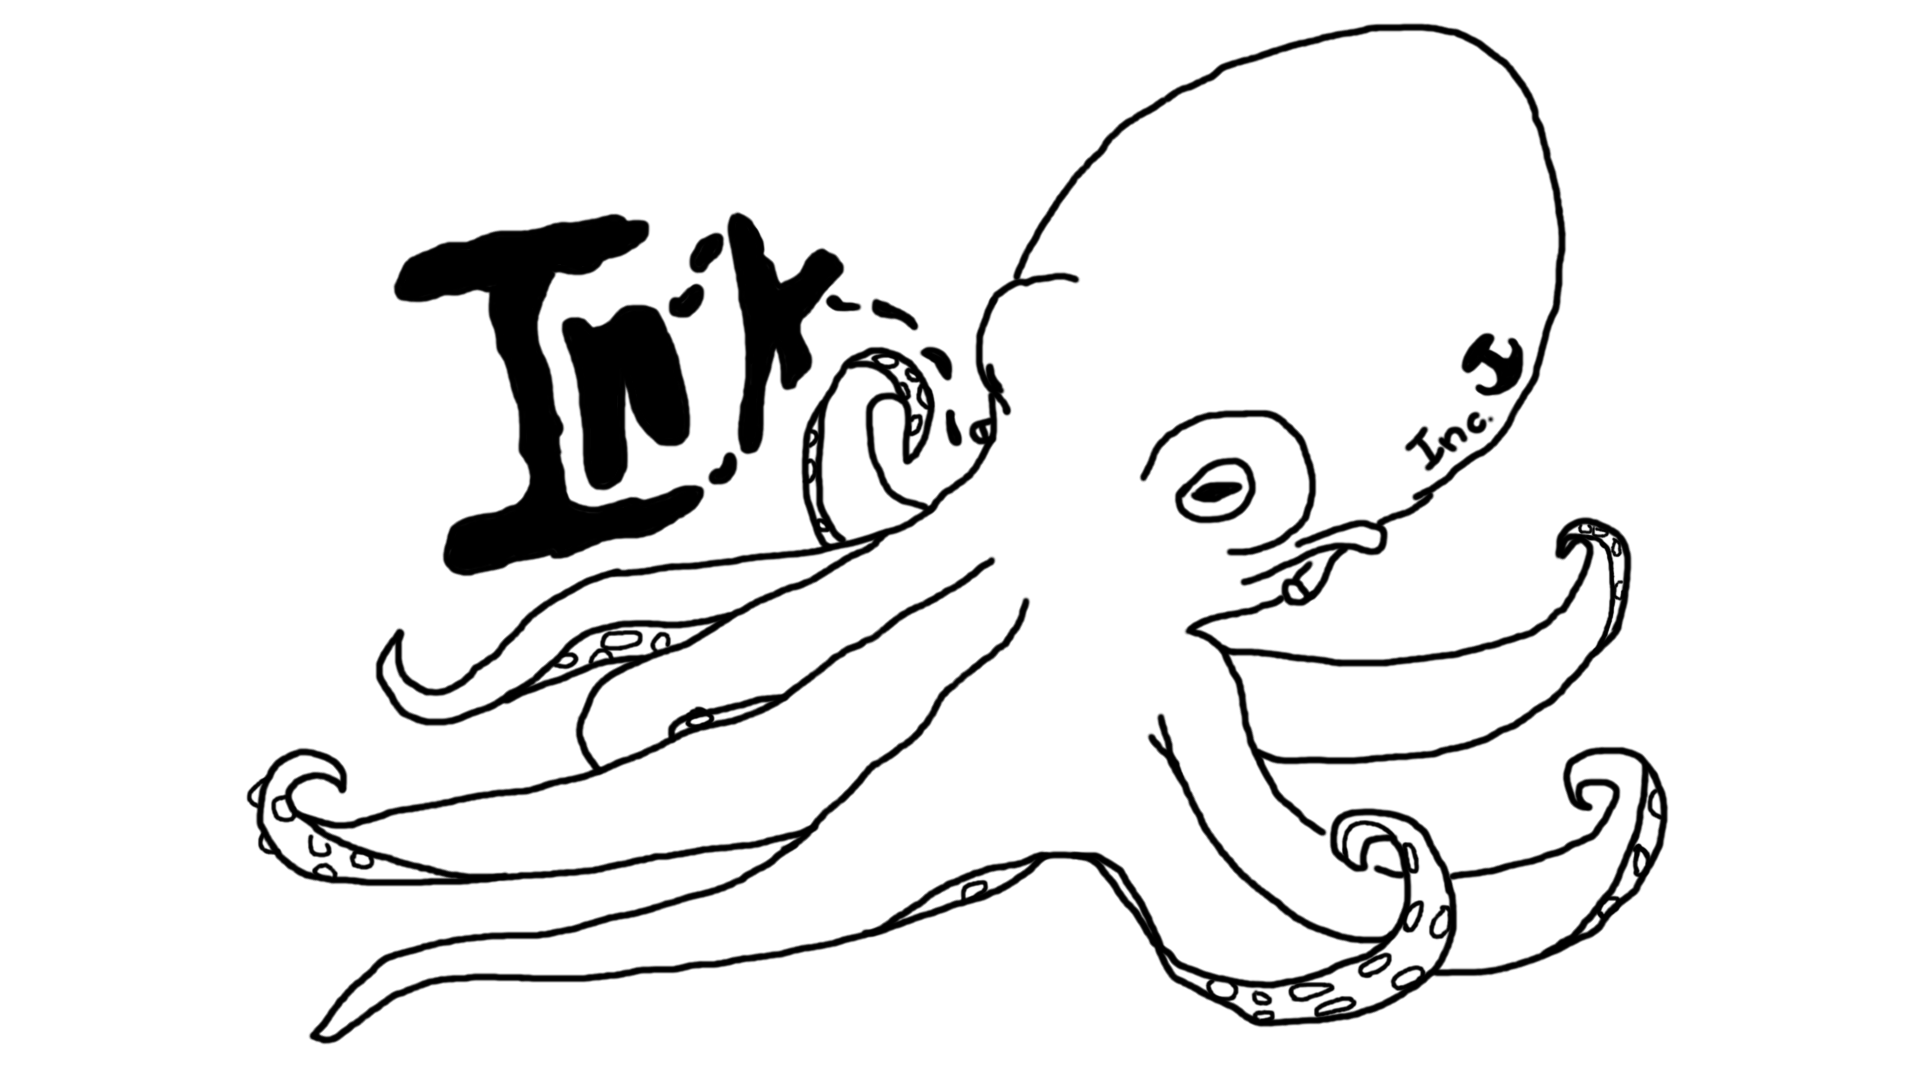
\includegraphics[height=3cm]{Abbildungen/logo.png}
%	\end{minipage}
%	\begin{minipage}{0.5\textwidth}
%		\flushright
%		Ink Inc.
%		\vspace{0cm}\\
%	\end{minipage}
	
	\centering
	\vfil
	\Large{\textbf{Stand {\today}}} \\ \bigskip
%	\normalsize{}
	\vfil
	\textsf{\textbf{\Huge{Wissenssammlung}}} \\ \bigskip
	\Large{\textbf{zur Übersicht der Geschichte von MMG der Ink Inc.}} \\
	\vfil
	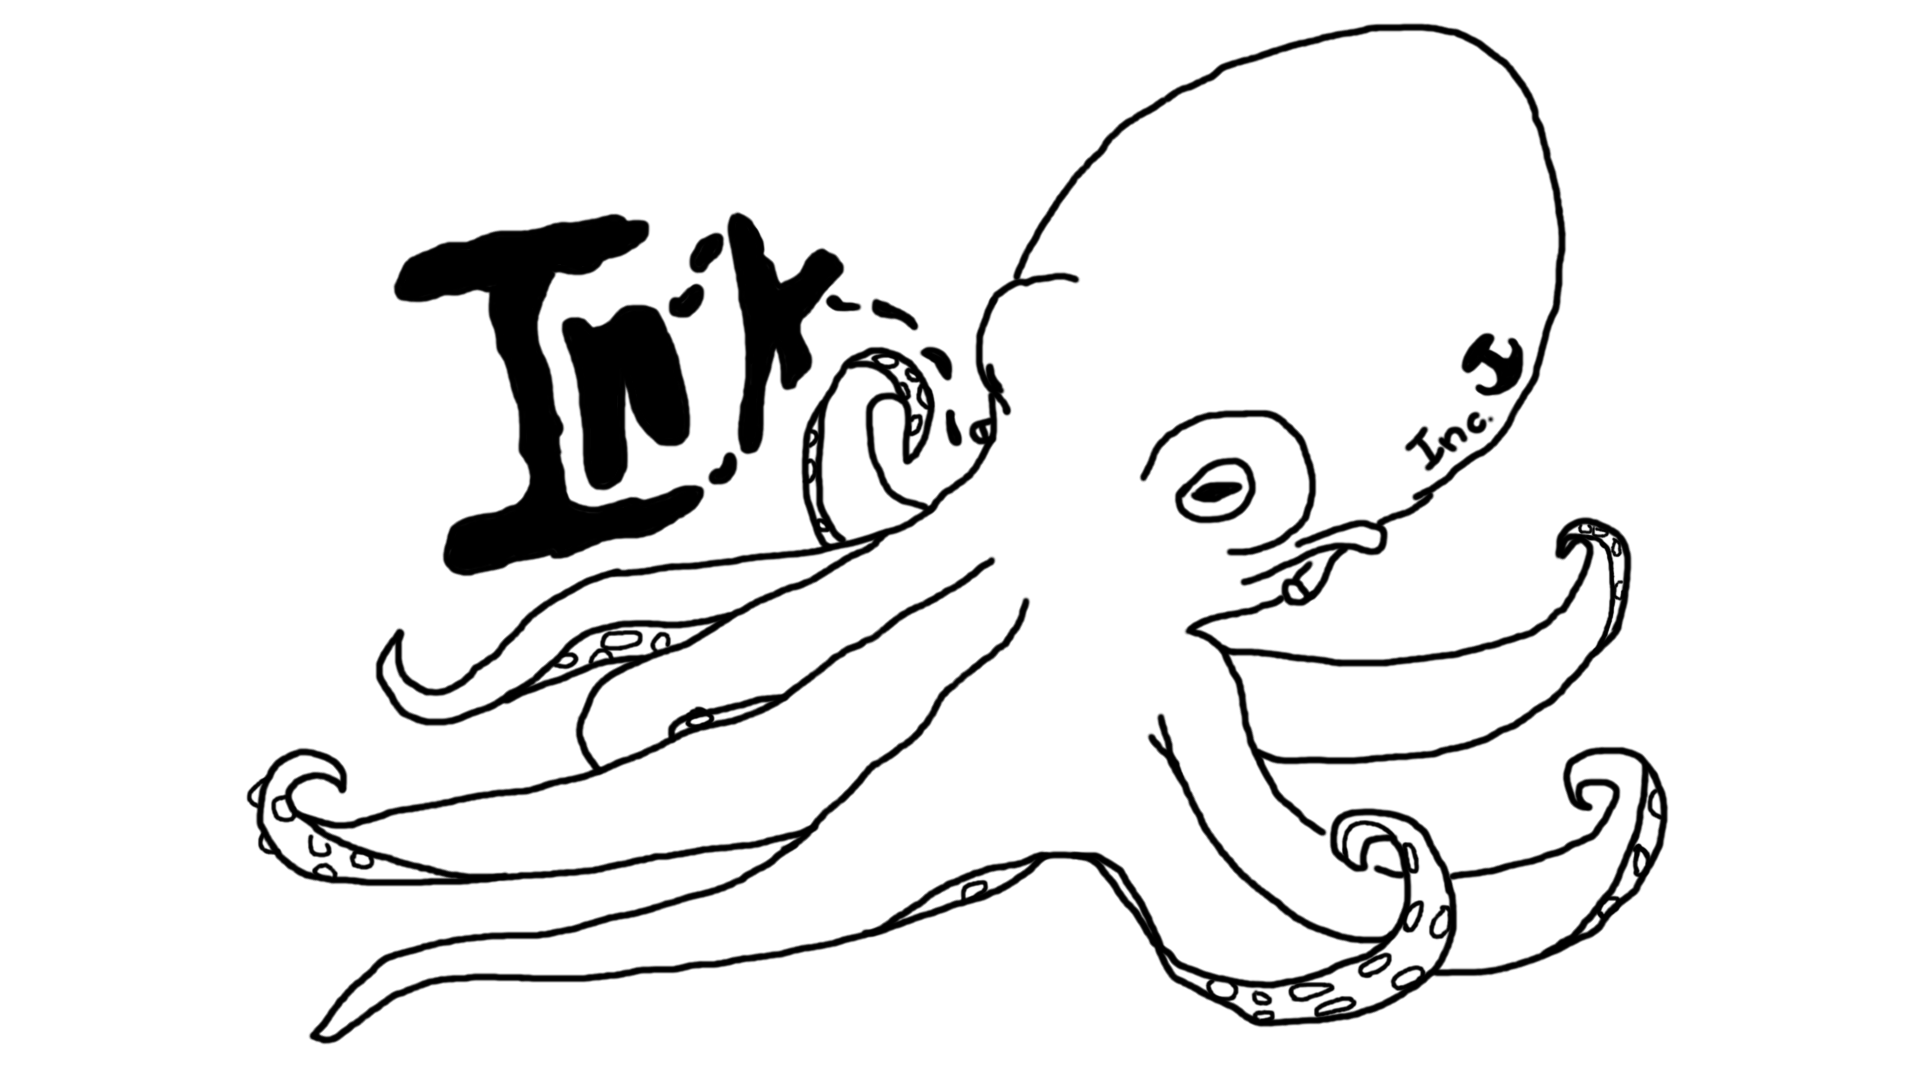
\includegraphics[width=\linewidth]{Abbildungen/logo.png}
	\vfil
	\large
	bearbeitet von\\
	Medsmiley, Thabb, Mine Schokokeks
\end{titlepage}

\pagenumbering{Roman}

\tableofcontents


%----------Inhalt-------------

%\include{Dateien/Welt}
%\include{Dateien/Land}
%\include{Dateien/Abenteuer}
%\include{Dateien/Spiel-Mechaniken}


%----------Anhänge------------


\end{document}